

\begin{frame}{\ft{Photo Viewer Interactive Cues}}

\doubleFrame{Color insertions switch from horizontal 
to vertical indicating which photos have been viewed 
(enlarged).  Separate and apart from that, the 
thumbnail of the current enlarged photo 
is marked with a thick colored border.  This border will 
surround the thumbnail and the overlay both for photos being 
viewed for the first time (with a horizontal color-band) 
and for photos being viewed a second time (with a vertical 
color-band).
}

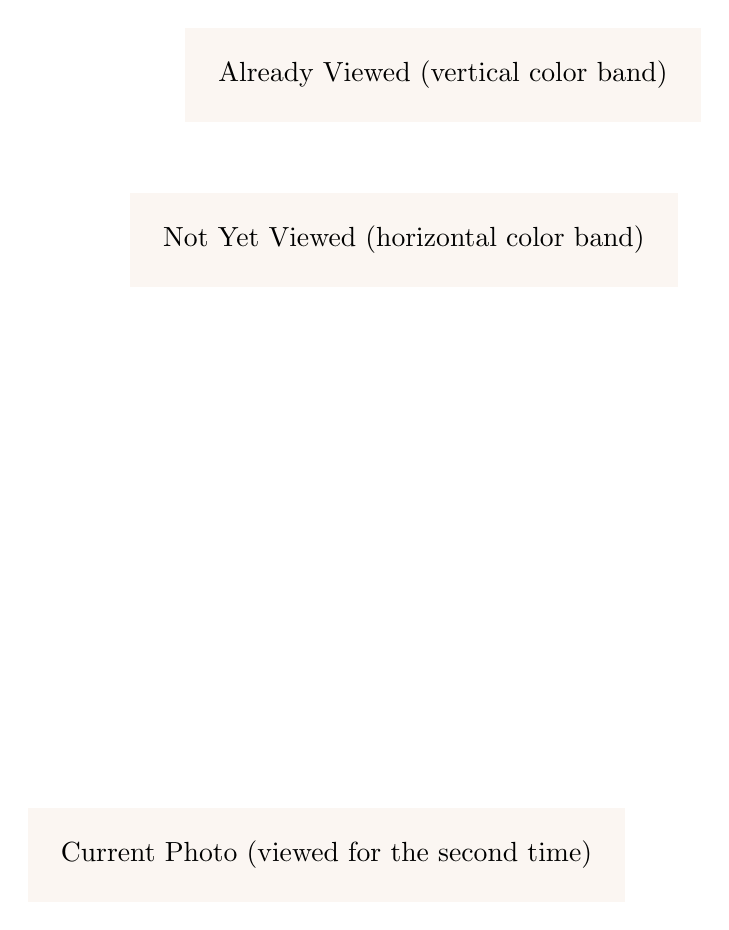
\begin{tikzpicture}
%\nodeincludegraphics[0.9\textwidth]{screenshots/ss-ph3.png}
\nodeincludegraphicsTR{5.5cm}{3.23cm}{screenshots/ss-ph3.png}

 %%\node [anchor=west] (note) at (11,11.2) {\Huge {\color{blGreen!30!black}Already Viewed}};

\node [anchor=west,fill=brown!8!white,inner sep=12, 
opacity=0.88, text opacity=1] (note) at (7,11.8) {\hc{Already Viewed (vertical color band)}};


%\ann{BlueGreen!30!red}{1}{.8mm}{blue!50!orange}{0.5}{3.61,8.95}{.4}{.6}{0.7}

\colorarr{>=latex, ->}{fcBoxColor!20!black}
{0.8}{darkRed!70!blue}{2}{1mm}{note.west}{3.7, 9}


\node [anchor=west,fill=brown!8!white,inner sep=12, 
opacity=0.88, text opacity=1] (note) at (6.3,9.7) {\hc{Not Yet Viewed (horizontal color band)}};

%\ann{BlueGreen!30!red}{1}{.8mm}{blue!50!orange}{0.5}{7.6, 7.3}{.73}{.35}{0.7}

%
\colorarr{>=latex, ->}{fcBoxColor!20!black}
{0.8}{darkRed!70!blue}{2}{1mm}{note.south}{8.2, 7.25}

%\node [anchor=west] (note) at (11,3) {\Huge {\color{blGreen!30!black}Current Photo}};

\node [anchor=west,fill=brown!8!white,inner sep=12, 
opacity=0.88, text opacity=1] (note) at (5,1.89) {\hc{Current Photo (viewed for the second time)}};

\colorarr{>=latex, ->}{fcBoxColor!60!black}
{0.8}{blGreen!30!red}{1}{1mm}{note.north west}{4.39, 4.75}


\end{tikzpicture}


\end{frame}

